\renewcommand{\vec}[1]{\textbf{#1}}

\chapter{Experimental Results}
\label{cha:experimental_results}

This chapter presents the experiments: first how accurately PCPG estimates the
expected prediction, then how well a logistic regression can be trained with PCPG
on incomplete data. Discussion of the results follow in
Chapter~\ref{cha:discussion}.

\section{Estimating the Expected Prediction}
\label{sec:results-estimate}

\paragraph{Setup.}
The data are generated with scikit-learn's \texttt{make\_classification}:
10{,}000 samples, of which half of the features are informative and the other
half are independent noise; 8{,}000 samples are used for training and 2{,}000 for
testing. The density $p(x)$ is a GMM with $K = 4$ diagonal components, fit on the
complete training points, and the classifier is a standard logistic regression from scikit-learn.
The number of features goes from $5$ to $5{,}000$, each one being
a factor $\sqrt{10}$ apart. For every test point a fraction
$\rho \in \{0.3, 0.5, 0.8\}$ of the features is hidden at random. 

MC and PCPG get the same budget of $1{,}200$ evaluations: MC draws $1{,}200$ samples, and PCPG uses
$M = 20$ Gauss--PG nodes and $N = 60$ Gauss--Hermite nodes. PCPG exact inner is PCPG
with the inner expectation in closed form (Section~\ref{subsec:gmm-exact-inner}),
so its error is that of the Gauss--PG rule alone. The error is the RMSE over 50 test
points against the exact value, which we compute from the Gaussian mixture of
$z \mid \xo$ (Section~\ref{subsec:gmm-direct}) with adaptive quadrature. 
The time is that of one batched call over all 2{,}000 test points on a GPU.

We run the comparison in two variants, which differ only in terms of 
standardisation and regularisation: one for the raw data with default regularisation $C = 1$, and one for the data with 
standardised features and stronger regularisation $C = 10^{-3}$. 
The standardisation is done on the training points, and the same transformation is applied to the test points. 
Some additional variants are in Appendix~\ref{app:estimate-variants}. 

\paragraph{Raw data, default classifier.}
We see that with only few features PCPG clearly outperforms MC by some orders of magnitude.
However after about $1000$ features, the error of PCPG grows rapidly and even gets larger than that of MC. 
Theories about why this happens are discussed in detail in Section~\ref{sec:accuracy-pcpg}, but 
the main reason is that the standard deviation of $z$ grows with the number of features, which makes 
the quadrature rules much less accurate.

\begin{figure}[H]
  \centering
  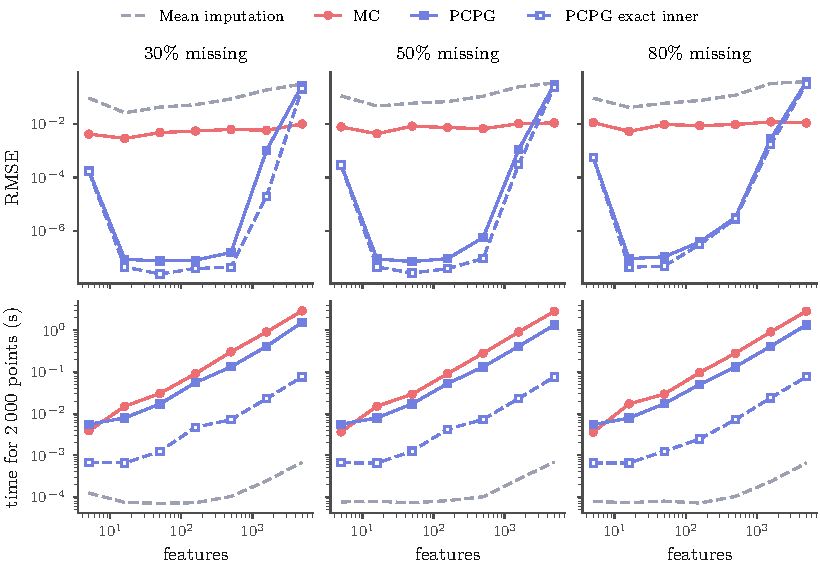
\includegraphics[width=\textwidth]{figures/estimate/gmm/comparison_0.5_20_60.pdf}
  \caption[Raw data, default classifier]{Raw data, logistic regression with
    $C = 1$.}
  \label{fig:comparison-default}
\end{figure}

\paragraph{Standardise data, stronger regularisation.}
The first idea is to standardise the features to mean $0$ and variance $1$ on the training points, and apply the same transformation to the test points.
This helps but does not completely solve the problem.
One also has to ensure that the magnitude of $w$ is controlled. The best way we found to do this, without changing the classifier too much, 
is to use different regularisation strengths $C$ for the logistic regression.
In (Table~\ref{tab:classifier-norm}) we show different values of $C$ and the resulting standard deviation of $z$ and test accuracy.

\begin{table}[H]
\centering
\caption[The logistic regression on standardised data]{The logistic regression on
the standardised data for different regularisations $C$: the standard deviation of
$z = w^T x$ over the training points and the accuracy on the test points.}
\label{tab:classifier-norm}
\renewcommand{\arraystretch}{1.2}
\begin{tabular}{rrrrrrr}
\hline
 & \multicolumn{2}{c}{$C = 1$} & \multicolumn{2}{c}{$C = 10^{-2}$} & \multicolumn{2}{c}{$C = 10^{-3}$} \\
$d$ & $\mathrm{sd}(z)$ & \textbf{test acc.} & $\mathrm{sd}(z)$ & \textbf{test acc.} & $\mathrm{sd}(z)$ & \textbf{test acc.} \\
\hline
5    & $3.70$  & $0.888$ & $2.50$ & $0.892$ & $1.12$ & $0.888$ \\
16   & $1.40$  & $0.721$ & $1.27$ & $0.721$ & $0.78$ & $0.713$ \\
50   & $2.14$  & $0.797$ & $1.80$ & $0.797$ & $0.99$ & $0.794$ \\
158  & $2.64$  & $0.805$ & $2.14$ & $0.805$ & $1.16$ & $0.798$ \\
500  & $3.07$  & $0.813$ & $2.36$ & $0.810$ & $1.25$ & $0.806$ \\
1581 & $5.43$  & $0.764$ & $2.88$ & $0.777$ & $1.36$ & $0.776$ \\
5000 & $12.42$ & $0.702$ & $3.79$ & $0.713$ & $1.65$ & $0.722$ \\
\hline
\end{tabular}
\end{table}

We see, that the stronger regularisation costs no accuracy:
from $d = 1581$ on, the test accuracy is even higher than with $C = 1$, which overfits there.

Then redoing the first experiment with standardised features and $C = 10^{-3}$, yields (Figure~\ref{fig:comparison-c1e3}),
and PCPG reaches an RMSE of about $10^{-7}$ in
every setting, clearly outperforming MC everywhere.  This shows, that the error of PCPG depends mainly
on the spread of $z$, not on the number of features. 
Whenever $z$ stays on a moderate scale, PCPG is accurate to about $10^{-7}$ for every $d$ and missing rate.

\begin{figure}[H]
  \centering
  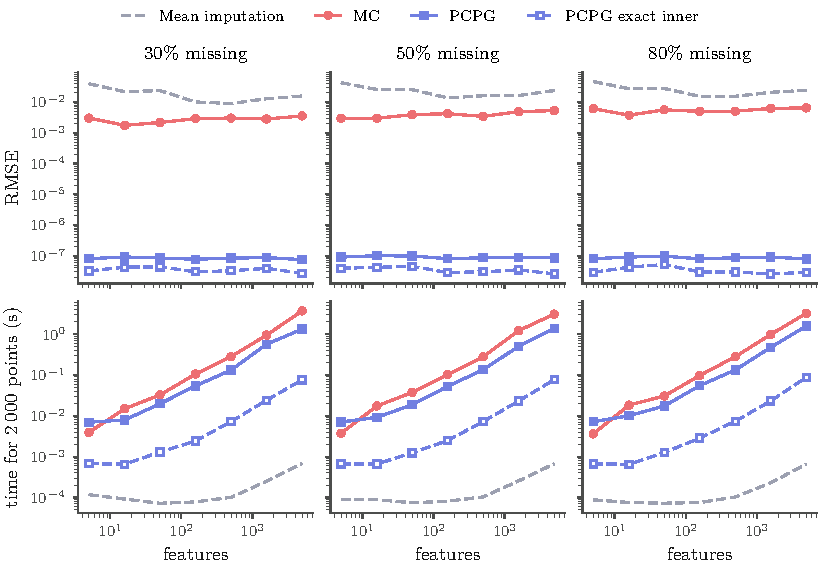
\includegraphics[width=\textwidth]{figures/estimate/gmm/comparison_0.5_20_60_norm_C1e3.pdf}
  \caption[Standardised data, $C = 10^{-3}$]{Standardised features, logistic
    regression with $C = 10^{-3}$.}
  \label{fig:comparison-c1e3}
\end{figure}

\paragraph{Runtime.}
The runtime for MC and PCPG it grows linearly in $d$, and from $d = 16$ on, PCPG is about twice as fast as MC at the same budget. 
PCPG exact inner needs no characteristic function and takes less than $0.1$\,s. 
Mean Imputation is of course the fastest. 

\clearpage

\section{Training with Missing Features}
\label{sec:training}

In this section we train a logistic regression on incomplete data with PCPG
inside the loss (Section~\ref{sec:training-pcpg}) and compare it against other typical
ways of training on incomplete data.

\subsection{Compared Models}
\label{subsec:training-models}

All models are again standard logistic regressions without intercept. They differ only in the
training points they see and in the prediction their loss is built from
(Table~\ref{tab:training-models}):
\begin{itemize}
  \item \textbf{Complete data:} an ordinary logistic regression from sklearn on the complete
        training points. It acts as an oracle, the classifier that training could reach if no features were missing. 
  \item \textbf{Mean imputation:} the same ordinary logistic regression on the training
        points with every missing feature replaced by the mean of its observed
        values.
  \item \textbf{MC, PCPG, Exact:} the expected marginal likelihood \eqref{eq:marginal-likelihood}
        on the incomplete training points, estimated by Monte
        Carlo, deterministic PCPG, or computed exactly. 
        Exact uses the direct route for Gaussian mixtures
        (Section~\ref{subsec:gmm-direct}) with Gauss--Hermite quadrature (a slightly higher error than adaptive quad, but much faster) for every
        component. 
\end{itemize}

\begin{table}[htb]
\centering
\small
\renewcommand{\arraystretch}{1.3}
\begin{tabular}{lll}
\hline
\textbf{Model} & \textbf{Training points} & \textbf{Prediction in the loss} \\
\hline
Complete data   & complete $x$                 & $\sigma(w^T x)$ \\
Mean imputation & $\xo$, $\xm$ filled by means & $\sigma(w^T x)$ \\
MC              & $\xo$                        & $\frac{1}{S}\sum_s \sigma(w^T x^{(s)})$ \\
PCPG            & $\xo$                        & PCPG, $M \times N$ nodes \\
Exact           & $\xo$                        & $\sum_k \tilde\pi_k(\xo) \E_{\mathcal{N}(m_k, v_k)}[\sigma(z)]$ \\
\hline
\end{tabular}
\caption{The compared models. The last three minimise the marginal likelihood
  \eqref{eq:marginal-likelihood}, the first two an ordinary logistic regression
  loss. All use the same $L_2$ penalty.}
\label{tab:training-models}
\end{table}

MC, PCPG and Exact are all trained with Adam on the same minibatches,
starting from $w = 0$, so that they differ only in the estimate of the
expectation. 

\subsection{Setup}
\label{subsec:training-setup}

The data for the experiment is setup exactly as in Section~\ref{sec:results-estimate}. 
The density is also again a GMM with $K = 4$ diagonal
components, now fit on the incomplete training points. PCPG uses $M = 20$
Gauss--PG nodes and $N = 60$ Gauss--Hermite nodes, and MC gets the same
budget of $S = 1{,}200$ samples per point and step. Exact uses 64 Gauss--Hermite
nodes per component. Adam runs for 100 epochs with minibatches of 1{,}024 points
and a learning rate of $0.01$.

We train one configuration with the raw data and default regularisation $C = 1$, 
and one with the standardised data and stronger regularisation $C = 10^{-3}$.

\subsection{Evaluation}
\label{subsec:training-evaluation}

The evaluation tries to answer two questions.
\begin{itemize}
  \item \textbf{How good is the training procedure?}
        MC, PCPG and Exact are trained identically. Any difference between
        their classifiers comes from how they estimate the expectation. We measure
        the mean absolute difference between the expected predictions of a
        classifier and those of the Exact classifier on the incomplete test points, where in the evaluation all are predicted exactly.
  \item \textbf{How good is the final classifier?} We want to see if the accuracy of
        $\sigma(w^T x)$ is on par with different training methods. 
        We compute the prediction accuracy once with complete test points 
        and once with partly missing test points. 
        For the incomplete test points, every model uses it's "own"
        rule:  mean imputation fill the missing features with
        their training means, MC, PCPG and Exact use their own estimate of the
        expected prediction and complete (training) data also uses the exact estimate.
\end{itemize}

\subsection{Results}
\label{subsec:training-results}

\begin{figure}[htb]
  \centering
  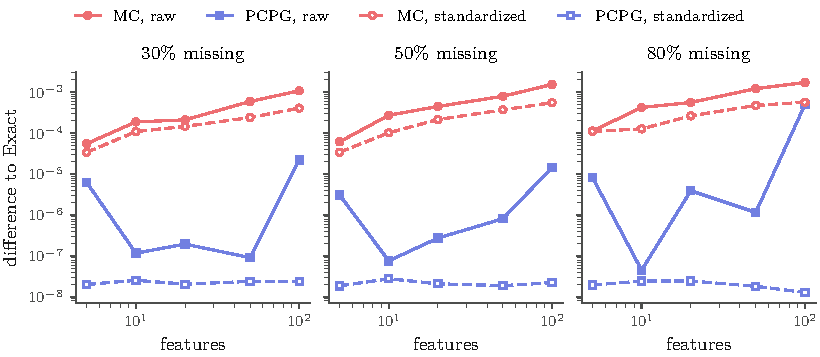
\includegraphics[width=\textwidth]{figures/train/gmm/comparison_0.5_20_60_difference.pdf}
  \caption[Difference to exact training]{Mean absolute difference between the
    expected predictions of the classifiers trained with MC and PCPG and those of
    the classifier trained with the exact expectation, on the incomplete test
    points, against the number of features $d$. Solid: raw data with $C = 1$,
    dashed: standardised data with $C = 10^{-3}$.}
  \label{fig:training-difference}
\end{figure}

\begin{figure}[htb]
  \centering
  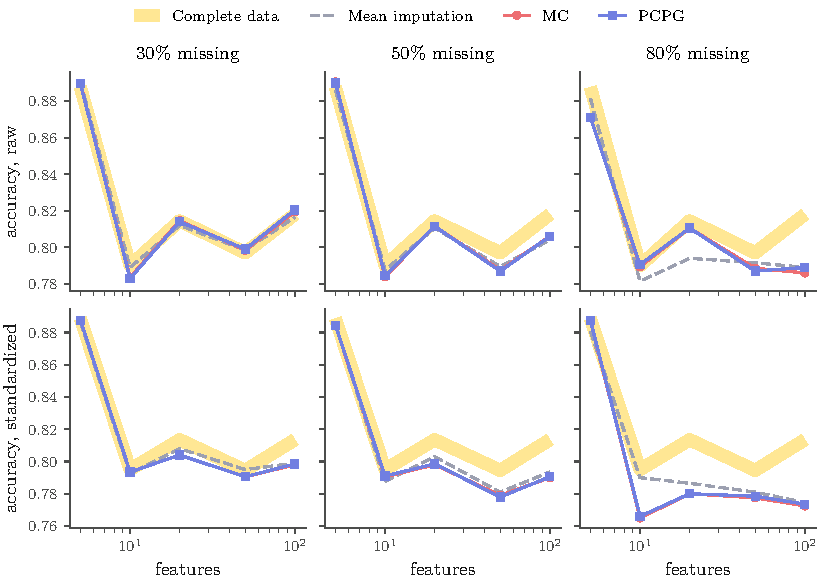
\includegraphics[width=\textwidth]{figures/train/gmm/comparison_0.5_20_60_accuracy_complete.pdf}
  \caption[Accuracy on complete points]{Accuracy of $\sigma(w^T x)$ on the
    complete test points against the number of features $d$. Top: raw data with
    $C = 1$, bottom: standardised data with $C = 10^{-3}$. The target is the
    classifier trained on complete data (yellow band).}
  \label{fig:training-complete}
\end{figure}

\begin{figure}[htb]
  \centering
  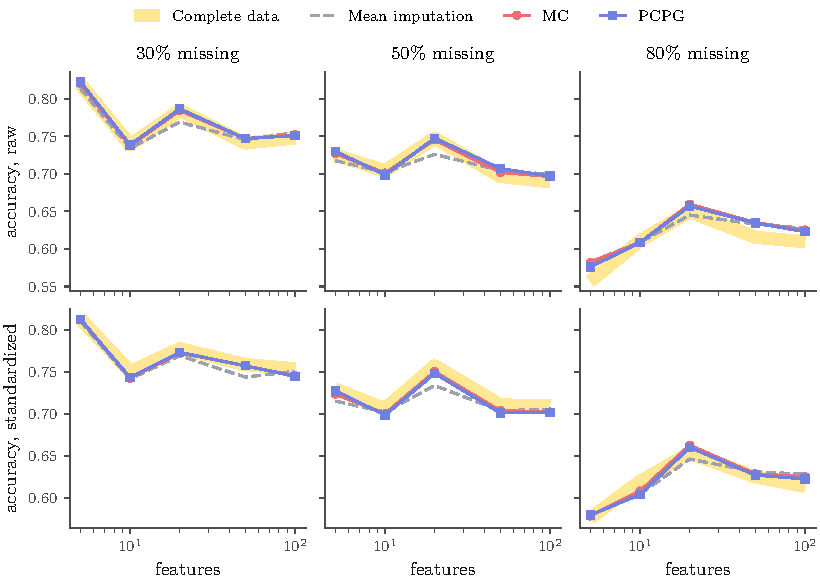
\includegraphics[width=\textwidth]{figures/train/gmm/comparison_0.5_20_60_accuracy_own.pdf}
  \caption[Accuracy on incomplete points, own rule]{Accuracy on the incomplete
    test points, every model with its own prediction rule: mean imputation for
    mean imputation, the estimated expected prediction for MC and PCPG. Top: raw
    data, bottom: standardised data. The target is the classifier trained on
    complete data with the exact expected prediction (yellow band).}
  \label{fig:training-own}
\end{figure}
